\section{Causal Impact: Motivations}\label{sec:motivations}

The central difficulty in causal attribution is not computing counterfactuals --- it is knowing which counterfactuals to compute, and recognising when a cause is merely blocked by context while still genuinely present.
Here a cause is \emph{blocked by context} when it is a genuine cause in general (it does produce the outcome in other situations) yet its causal path was inactive in the particular case at hand, so it made no difference to what actually happened.
This is the distinction between \emph{type} causation (does $X$ tend to cause $Y$?) and \emph{token}, or actual, causation (was $X$'s contribution live in the specific situation we are explaining?); methods built for the former routinely miss the latter, which is the gap the running example below makes concrete.
There are principled probabilistic theories of type-level causal strength --- \citet{sprenger2018foundations}, for instance, derives a difference-making measure $p^*(E \mid C) - p^*(E \mid \neg C)$ axiomatically --- but they deliberately bracket the token-level question of which cause was live in the case at hand, and amalgamate over mediators just where the context-sensitivity we are after requires tracking them.
The closest predecessors of this approach, none individually achieve all of this: actual causality handles context sensitivity but is computationally intractable and not general enough;
the probability of necessity and sufficiency scales well, but lacks context sensitivity.
This section builds intuition for both limitations through a running example, setting up the design choices that motivate \ourapproach in Section~\ref{sec:causal_impact}.
We first revisit Halpern's actual-cause
construction on a deterministic Old Boys' Club Bank (OBCB) example to see what witnesses do and why a plain
but-for clause misses Alice's case. We then turn to Pearl's PN/PS/PNS on a stochastic
OBCB to introduce the probabilistic machinery actual causality lacks, while showing
that, without witnesses, PN/PS/PNS cannot register Alice's missing credit check. We
close with a ``Path forward'' subsection that distils what \ourapproach must inherit
from each predecessor before Section~\ref{sec:causal_impact} formalises it.

\subsection{Actual Causality}

Consider the following (deterministic, discrete) model:

\begin{example}[Bob at Old Boys' Club Bank]
Bob applied for a home mortgage loan with the local branch of OBCB, and his application was denied.
The OBCB policy requires applicants to pass a credit score check, but it only performs this check if the applicant is male; all non-male applicants are rejected outright. \label{ex:obcb} Thus, the procedure is:
\begin{align*}
\varname{check} &= (\varname{gender} = \text{male}) \\[4pt]
\varname{check\text{-}failed} &= \varname{check} \land (\varname{credit} = \text{bad}) \\[4pt]
\varname{loan} &= \lnot \varname{check\text{-}failed} \land (\varname{gender} = \text{male})
\end{align*}
\end{example}

\noindent Why was Bob’s loan application denied?
An intuitive explanation is that his credit was bad: had it been good, the outcome would have been different.
In contrast, his gender does not appear to be responsible for the rejection: had it been different,
his application still would have been denied (albeit this time due to $\varname{check}=F$).

This suggests a counterfactual approach to feature responsibility attribution: perhaps we can identify the features responsible for a particular outcome by asking counterfactual questions: would the outcome have been different if a specific feature had a different value?
This is called the \textit{but-for clause}: Bob wouldn’t have been denied the loan but for his bad credit.

Concretely, consider a model $M$ with \emph{exogenous variables} $\mathbf{U}$, which are the source of stochasticity, and \emph{endogenous variables} $\mathbf{V}$,  which are influenced by other variables in the model. 
Let $\mathbf{S} \subseteq \mathbf{V}$ be the variables we suspect to be causally responsible (call them \emph{causal suspects}), and 
$Y \in  \mathbf{V}$ be an outcome of interest. 
Suppose we consider only one suspect $S \in \mathbf{S}$ and mark factual values with $^\star$. 
Under a setting $\mathbf{U} = \mathbf{u}$ of the exogenous variables, $M$ produces $S = s^\star$ and $Y = y^\star$, denoted $(M, \mathbf{u}) \vDash S=s^\star, Y=y^\star$. We read $\vDash$ as ``yields'' (the model under noise $\mathbf{u}$ makes the stated equalities true), and its crossed form $\not\vDash$ as ``does not yield'' (the stated event fails to hold).
We call this the \emph{factual} scenario.
An intervened model where a variable $S$ is set to an alternative value $s'$ is denoted $(M, \mathbf{u})[S \leftarrow s']$.

A first attempt at defining a counterfactual notion of causal responsibility,
following the counterfactual-dependence tradition \citep{lewis1973causation,
actualCausalityHalpern}, is:
\begin{definition}[But-for, single]
$S=s^\star$ is causally responsible for  $Y=y^\star$  in $(M, \mathbf{u})$ if and only if $(M, \mathbf{u}) \vDash S=s^\star, Y=y^\star$ and $(M, \mathbf{u})[S \leftarrow s'] \not \vDash Y=y^\star$ for some $s' \neq s^\star$.
\end{definition}

\noindent 
In a given context, $S$ is causally responsible for an outcome only when intervening on $S$ with some alternative value would change that outcome. 
Bob’s credit score satisfies this condition: had his credit score been higher, the loan might have been approved. 


However, this cause test is too coarse. Consider another case:
\begin{example}[Alice at OBCB] 
Alice is a woman with bad credit.
She applies for a loan with OBCB and is rejected.
\end{example}
\noindent Why was Alice denied the loan?
Under the but-for clause for single cause candidates, neither her gender nor her credit score are responsible.
No matter how high her credit score, her application would still have been denied because the bank does not, effectively, loan to women.
Had her gender been different, she would still have been denied for having bad credit.

To address this example, we could consider sets of factors as causes:
\begin{attempt}[But-for, sets]
Variables $\mathbf{C}\subseteq \mathbf{S}$ with factual values $\mathbf{C} = \mathbf{c}^\star$ 
are causally responsible for $Y = y^\star$ in $(M, \mathbf{u})$ if and only if 
$(M, \mathbf{u}) \vDash \mathbf{C} = \mathbf{c}^\star, Y = y^\star$ and $(M, \mathbf{u})[\mathbf{C} \leftarrow \mathbf{c'}] \not \vDash Y= y ^\star$ for some $\mathbf{c'}$ everywhere different from $\mathbf{c}^\star$, where no proper subset of $\mathbf{C}$ has this property. 
\end{attempt}

\noindent The minimality condition reflects our preference for explanations that include only relevant properties.

Under this generalization, the set  $\mathbf{c}^\star = \{\varname{gender}=\text{female}, \varname{credit}=\text{bad}\}$
 is jointly responsible for Alice's application being denied because 
 there exists $\mathbf{c}' = \{\varname{gender}=\text{male}, \varname{credit}=\text{good}\}$ that would change the decision
and $\mathbf{c}^\star$ is minimal; neither gender nor credit alone would have changed the decision. But what can we say about the individual features? 
We could say that the whole set bears responsibility but individual features do not, or that any feature in a cause set is partially and equally accountable.
Both approaches have issues, as they imply the features are equally responsible.
This conflicts with our intuition: OBCB did not evaluate Alice’s credit score, so her denial was caused by her gender.
This verdict does not rest on counterfactual reasoning alone. Tracing the model on Alice's inputs, her denial is produced through the $\varname{gender}$ term of the $\varname{loan}$ equation, while $\varname{credit}$ enters only through $\varname{check\text{-}failed}$, which is false and never propagates to the outcome, so on a production (causal-process) view of causation \citep{hall2004two}, credit transmits no influence to Alice's denial at all.
The counterfactual and production traditions thus converge on this assessment, so the attribution is not an artifact of one chosen formalism.

The structural pattern is what the actual-causality literature calls
\emph{preemption} (sometimes \emph{undercutting})~\citep{lewis1973causation,
actualCausalityHalpern}: two distinct causal routes
might each have been sufficient to produce the outcome, but only one is actually
engaged, with the other prevented from operating.
Alice's gender preempted her credit by preventing the check from happening, so
credit had no chance to act.
The closely related notion of \emph{over-determination}~\citep{paulhall2013,
actualCausalityHalpern} covers cases in which
multiple sufficient causes coexist without one preempting the other (e.g., two
simultaneous fatal shots).
Both phenomena defeat a simple single-cause but-for test, since intervening on any one of the
candidate causes leaves the outcome unchanged.\footnote{
The canonical preemption example: Jim is both stabbed and poisoned, and dies.
Stabbing works quickly, so it kills Jim before the poison takes effect, and the
stabbing caused his death.
But-for clauses fail to break the symmetry here as well: removing the stabbing
leaves Jim dead by poison, and removing the poison leaves him dead by stab.
}

Prior work suggests a way out of this difficulty: hold some of the context in which counterfactuals are evaluated fixed, 
calling such fixed variables \emph{witnesses}.
Let us focus on the mediator $\varname{check\text{-}failed}$ between $\varname{gender}$ and $\varname{loan}$.
If we fix this variable at the factual value by intervening, then counterfactually, Alice would have been granted the loan if she were male.
However, there is no context fixed at the actual value such that, had her credit score been higher, she would have been granted the loan.
Enumerating the candidate causes, their counterfactual treatments, the witness held fixed, and the resulting outcome makes the test concrete (Alice's factual run is $\varname{gender}{=}\text{female}$, $\varname{credit}{=}\text{bad}$, giving $\varname{check\text{-}failed}{=}0$ and $\varname{loan}{=}\text{denied}$):

\begin{center}
\begin{tabular}{llll}
\toprule
Candidate cause $\mathbf{C}$ & Treatment $\mathbf{c}'$ & Witness $\mathbf{T}=\mathbf{t}^\star$
  & Outcome ($\varname{loan}$) \\
\midrule
$\varname{gender}{=}\text{female}$ & ${\to}\,\text{male}$ & $\varname{check\text{-}failed}{=}0$
  & denied $\to$ \textbf{granted} \\
$\varname{gender}{=}\text{female}$ & ${\to}\,\text{male}$ & none (recomputed)
  & denied $\to$ denied \\
$\varname{credit}{=}\text{bad}$    & ${\to}\,\text{good}$ & any
  & denied $\to$ denied \\
\bottomrule
\end{tabular}
\end{center}

\noindent Fixing the mediator $\varname{check\text{-}failed}$ at its factual value reveals
$\varname{gender}$ as an actual cause (row~1); without the witness the intervention recomputes the
mediator and the outcome does not flip (row~2); no witness makes $\varname{credit}$ a cause (row~3).
This motivates the following formalization:
\begin{definition}[Actual cause (modified Halpern--Pearl)]\label{def:ac_intuitive}
Let $\mathbf{S}\subseteq\mathbf{V}$ be a suspect pool and
$\mathbf{W}\subseteq\mathbf{V}$ a witness pool, observed in $(M,\mathbf{u})$ at
factual values $\mathbf{S}=\mathbf{s}^\star$ and $\mathbf{W}=\mathbf{w}^\star$.
A cause set $\mathbf{C}\subseteq\mathbf{S}$ at its factual setting
$\mathbf{C}=\mathbf{c}^\star$ is an \emph{actual cause} of $Y=y^\star$ in
$(M,\mathbf{u})$ if there is a witness set $\mathbf{T}\subseteq\mathbf{W}$
disjoint from $\mathbf{C}$ such that:
\begin{itemize}[itemsep=2pt,topsep=2pt,parsep=0pt]
    \item \textbf{Factivity.} The cause, the witness pool, and the outcome
    are all observed at their factual values:
    \[ (M,\mathbf{u})\vDash \mathbf{C}=\mathbf{c}^\star,\;
                              \mathbf{W}=\mathbf{w}^\star,\;
                              Y=y^\star. \]
    \item \textbf{Witnessed necessity.} Holding $\mathbf{T}$ at its factual
    setting $\mathbf{t}^\star$ while intervening on the cause overturns the
    outcome, for some alternative $\mathbf{c}'$ distinct everywhere from
    $\mathbf{c}^\star$:
    \[ (M,\mathbf{u})\bigl[\mathbf{C}\leftarrow\mathbf{c}',\;
                            \mathbf{T}\leftarrow\mathbf{t}^\star\bigr]
        \not\vDash Y=y^\star. \]
    \item \textbf{Minimality.} No proper subset of $\mathbf{C}$ satisfies the
    two conditions above.
\end{itemize}
\end{definition}

\noindent Definition~\ref{def:ac_intuitive} is Halpern's \emph{modified} definition of actual
causality \citep{halpern2015modification, actualCausalityHalpern}, specialized to an explicit suspect
pool $\mathbf{S}$ and witness pool $\mathbf{W}$. \ourapproach uses Halpern's modified definition, with witnesses held at their actual values; prior probabilistic extensions of actual causation instead build on the original Halpern--Pearl definition (Section~\ref{sec:other-prob-ac}).
This definition extends but-for causality with a witness set $\mathbf{T}$ that is fixed to its factual value by
an intervention.
Under this definition, to determine the cause of an outcome, we need to find a cause set $\mathbf{C}$, alternative values 
$\mathbf{c}'$ (trivial if the variables are binary and less so if they are categorical or continuous),
and a witness set $\mathbf{T}$.
$\mathbf{C}$ and $\mathbf{T}$ are drawn from sets of size at most $2^{|\mathbf{V}|}$, so a brute-force computation
 is expensive.

\noindent The witnessed-necessity template above is the Halpern--Pearl definition, which has
been refined considerably since: \citet{beckersPrincipled2018} rebuild actual causation from a
production/dependence pair, \citet{beckersTransitivity2017} chart when it is (in)transitive and
asymmetric, and \citet{beckersSufficiency2021,beckersNESS2021} ground it in NESS-style sufficient
sets, where a cause is a necessary element of a set that suffices for the outcome; and
\citet{beckers2025nondeterministic} most recently extends it to nondeterministic
structural models. We build on the
same witnessed-necessity core, but --- anticipating the probabilistic turn below --- read its two
halves, necessity under intervention and sufficiency of the held-fixed configuration, as graded
quantities, not a single binary verdict.

Putting computational difficulties aside, the deeper limitation of the
construction so far is that it lives entirely in deterministic models.
Real-world attribution problems are typically probabilistic: policies apply
with some probability, mechanisms occasionally fail or are overridden, and the
analyst usually wants to reason about the unit-level outcome in the presence
of this noise.
One can, of course, place a distribution over the exogenous noise $\mathbf{u}$ and read
off the probability of the actual-cause verdict; this is the route taken by Pearl's
probability of causation \citep{causalityPearl} and by the degree-of-blame and harm
constructions of Chockler, Halpern, and Beckers
\citep{chocklerResponsibilityBlameStructuralModel2004, beckersHarm2022,
beckersQuantifyingHarm2023}.
The result is a probabilistic envelope around the same binary kernel, with the same computational demands.
This construction --- Pearl's \emph{probability of actual causation}
\citep[Def.~10.3.5]{causalityPearl} --- is also the closest neighbour of \ourapproach{}
and agrees with it in simple cases, so we defer a precise side-by-side comparison to
Section~\ref{sub:pearl_actual_cause_prob}. This is one of the reasons we
turn next to a different family of attribution tools.

\subsection{Probability of Necessity and Sufficiency}

To bring probability into the picture, we now consider a stochastic variant of the
OBCB example in which the bank's gendered policies apply only with some probability:
women are checked only sometimes, men are skipped only sometimes, and even when
the check happens its outcome is occasionally overridden by loan-officer
discretion. This is the natural setting for Pearl's probabilities of necessity,
sufficiency, and their conjunction (PN, PS, PNS)
\citep{pearl1999probabilities,tian2000probabilities},\footnote{Probabilities of
causation have also been put to work outside token-level attribution:
\citet{wangJordanDesiderata2021} formalize representation-learning desiderata ---
non-spuriousness, efficiency, and disentanglement --- as computable criteria built
from probabilities of causation, paralleling our use of the same primitives for
feature attribution.} which we introduce in this
subsection. As we will see, these scale gracefully into the stochastic regime
but, without an analogue of the witness mechanism, mis-attribute Alice's denial.

\begin{example}[OBCB, stochastic]\label{ex:obcb_stochastic}
The bank performs credit checks for a randomly selected 20\% of women and skips checks for a randomly selected 10\% of men.
Unchecked applicants are rejected.
Furthermore, if a man's credit check fails, he is nevertheless accepted 5\% of the time and if a woman's credit check succeeds, she is denied 10\% of the time.
We assume that the population is evenly divided into male and female and good and bad credit.
Formally, the model, using 1 for male and 1 for good credit, is:

\begin{align*}
\varname{loan-prob}(\varname{gender}, \varname{check\text{-}failed}) &=
\begin{array}{r|cc}
 & \varname{check\text{-}failed}{=}0 & \varname{check\text{-}failed}{=}1 \\ \hline
\varname{gender}{=}0 & 0.9 & 0 \\[2pt]
\varname{gender}{=}1 & 1   & 0.05
\end{array}
\\[6pt]
\varname{credit} &\sim \mathrm{Bern}(0.5) \\
\varname{gender} &\sim \mathrm{Bern}(0.5) \\
\varname{check} \mid \varname{gender}
   &\sim \mathrm{Bern}\bigl((1-\varname{gender}) \cdot 0.2
                            + \varname{gender} \cdot 0.9\bigr) \\
\varname{check\text{-}failed} &= \varname{check} \cdot (1-\varname{credit}) \\
\varname{loan\text{-}if\text{-}checked}
   \mid \varname{gender}, \varname{check\text{-}failed}
   &\sim \mathrm{Bern}\bigl(\varname{loan-prob}(\varname{gender},
                                                \varname{check\text{-}failed})\bigr) \\
\varname{loan} &= \varname{loan\text{-}if\text{-}checked} \cdot \varname{check}
\end{align*}
\end{example}

\begin{figure}[htbp]
\centering
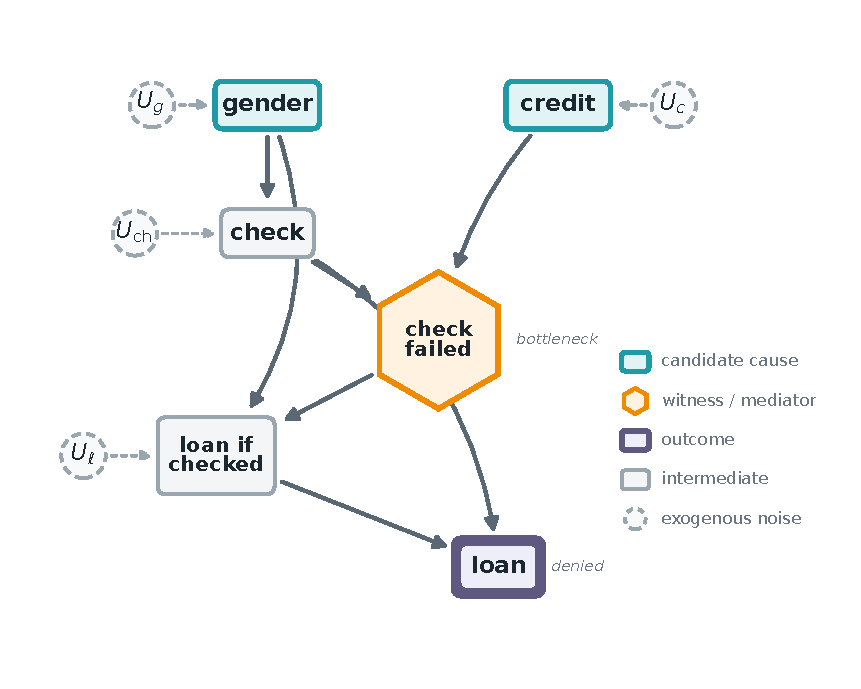
\includegraphics[width=0.62\linewidth]{figures/dag_obcb.pdf}
\caption[OBCB causal structure]{Causal structure of the OBCB loan model
(Example~\ref{ex:obcb_stochastic}). Node shape and colour encode role: the
\emph{candidate causes} \varname{gender} and \varname{credit} (teal boxes), the
\emph{witness} \varname{check-failed} (gold hexagon), and the \emph{outcome}
\varname{loan} (purple double box); intermediate variables are grey. Dashed circles
are the exogenous noise $U_V$ feeding each \emph{stochastic} mechanism---the
deterministic nodes \varname{check-failed} and \varname{loan} carry none. Note that
\varname{check} reaches \varname{loan} along two routes: through the
\varname{check-failed} bottleneck and directly as the screening gate
($\varname{loan}=\varname{loan-if-checked}\cdot\varname{check}$). \ourapproach holds
the bottleneck witness fixed to keep these two routes distinct.}
\label{fig:dag_obcb}
\end{figure}

\noindent The witness mechanism works well for deterministic models, but actual causality
in its standard form offers no straightforward way to handle probabilistic ones. Before
extending the witness idea to the stochastic setting, it is instructive to examine a
probabilistic approach that scales more naturally --- Pearl's probabilities of necessity
and sufficiency \citep{pearl2022probabilities} --- and to ask what it would miss without
witnesses. This will let us identify what probabilistic machinery is needed, and what
context-sensitivity is lost when witnesses are absent, motivating the synthesis that
\ourapproach provides.
The following definitions allow for probabilistic models, but assume that all variables are Boolean (PCI will relax this assumption,
 allowing for continuous variables).
Pearl considers two ways that a cause may relate to an effect: it may be necessary or sufficient for the effect.
A cause is necessary if, counterfactually absent the cause, the effect is unlikely to occur; it is sufficient
if the effect is counterfactually likely in the presence of the cause.
We now formalize these ideas and discuss them in the context of the running example.

\begin{definition}[Probability of Necessity]
Let the probability of necessity \citep{pearl1999probabilities} be the probability that the outcome $Y=y$ would not have occurred in the absence of  $C = c^\star$, given that both occurred: \[\pn(C = c^\star, Y = y^\star) = P\!\left(Y_{c'} \neq y^\star \;\middle|\; C = c^\star, Y = y^\star\right),\] where $Y_{c'}$ is the value of $Y$ after intervening on $C$ with $c'\neq c^\star$.\footnote{Read in twin-network fashion \citep{balke1994probabilistic, causalityPearl}: one draws an exogenous noise $\mathbf{u}\sim P_{\mathbf{U}}$, computes the factual $Y$ under the unintervened structural equations and the counterfactual $Y_{c'}$ under the intervened equations, and conditions on the joint event $\{C=c^\star,Y=y^\star\}$. Both $Y$ and $Y_{c'}$ live on the same probability space and share the same $\mathbf{u}$.}
\end{definition}

Strictly speaking, the probability of necessity is less specific to a particular situation than the actual-cause test above: as written, it conditions only on the cause--outcome pair, so it asks whether being male causes \emph{someone} to be denied, not whether it caused \emph{Bob} --- whose bad credit we already know --- to be denied.
We therefore report two readings.
The \emph{population-level} value conditions only on the cause and outcome, exactly as the definition prescribes.
The \emph{individual-level} value additionally conditions on the subject's other observed features (for Bob, on $\varname{credit}=\text{bad}$), specializing the query to that person.
The individual-level reading is the one closer to actual causation; we report both throughout, and the same population/individual split applies to $\ps$ and $\pns$ below.


We illustrate the computation for Alice's gender. Alice is factually
$\varname{gender}=\text{female}$, $\varname{credit}=\text{bad}$,
$\varname{loan}=F$; the counterfactual intervenes to set
$\varname{gender}=\text{male}$ while leaving $\varname{credit}=\text{bad}$.
Tracing the male-intervention branches through the model
(Appendix~\ref{app:obcb}, \S\ref{app:obcb_pn}) gives
$\pn(\varname{gender}=\text{female}, \varname{loan}=F \mid \text{Alice})
= 0.9 \cdot 0.05 = 0.045$.
Computing the analogous quantities for the remaining (variable, person) pairs gives
the individual-level values shown in Table~\ref{tab:pn_ps_pns}; the table also lists
population-level values for comparison.

The PN scores partially align with intuition: Bob's bad credit is high
($\pn=0.90$), and his gender score is zero, matching the reading that his gender played
no role.
But Alice's PN values do not separate gender (0.045) from credit (0.18)
particularly well, and Alice's gender PN is only marginally above Bob's, not the
sharp distinction we would want, given that the bank never even evaluated Alice's
credit.
PN cannot register this asymmetry: it asks counterfactually what would happen
under intervention without any context about which causal paths were active.
For the full picture we need a second quantity, the probability of sufficiency.

\begin{definition}[Probability of Sufficiency]
Let the probability of sufficiency be the probability that the outcome $Y=y^\star$ would have occurred in the presence of $C = c^\star$, given that neither $C=c^\star$ nor $Y=y^\star$ occurred:
\[\ps(C = c^{\star}, Y = y^\star) =  P\!(Y_{c^\star} = y^\star \;\vert\;  C = c',\ Y \neq y^\star)\]
where $c' \neq c^\star$ and $Y_{c^{\star}}$ is the value of $Y$ after intervening on $C$ with $c^\star$.
\end{definition}

To query whether the factual cause was sufficient, we condition on the counterfactual: we assume the cause did \emph{not} take its factual value and the outcome did \emph{not} occur, then intervene to restore the factual cause value and ask whether the outcome now occurs.
Intuitively, this asks: if the cause had been absent and things had gone differently, would reinstating the cause have brought the outcome about?
Let's look at the resulting values. 

We illustrate $\ps$ for Alice's gender. Following the same convention as for
$\pn$, the individual-level computation additionally conditions on Alice's
credit ($\varname{credit}=\text{bad}$): we fix her credit but flip the cause and
outcome to their non-factual values ($\varname{gender}=\text{male}$,
$\varname{loan}=T$), then intervene to restore $\varname{gender}=\text{female}$
and ask whether the loan is again denied. Both check branches yield
$\varname{loan}=F$ (Appendix~\ref{app:obcb}, \S\ref{app:obcb_ps}), so
$\ps(\varname{gender}=\text{female}, \varname{loan}=F \mid \text{Alice}) = 1$.
The remaining individual values, along with population-level values for comparison,
appear in Table~\ref{tab:pn_ps_pns}.
Two cases warrant comment: Bob's gender PS is undefined because the required
conditioning event ($\varname{gender}=\text{female}$, $\varname{credit}=\text{bad}$,
$\varname{loan}=T$) has probability zero in the model; Bob's credit PS is $0.955$
rather than $1$ because the model includes a $5\%$ exception rate for males who fail
the credit check.


To combine the insights of the two scores, we would like to find causes that are both necessary and sufficient.
This notion is  formalized as follows:

\begin{definition}[Probability of necessity and sufficiency]
Let the probability of necessity and sufficiency be the probability that the outcome $Y=y^\star$ would have occurred in the presence of $C = c^\star$ and that it would not have occurred under the intervention $C=c'$:
\[\pns(C = c^{\star}, Y = y^\star) =  P\!(Y_{c^{\star}} = y^\star, Y_{c'} \neq y^\star ).\]
This quantity factorises into a weighted sum of $\pn$ and $\ps$ by the
consistency rule of counterfactuals
\citep[\S 9.2]{causalityPearl}:
\[
  \begin{aligned}
    \pns(C = c^\star,\, Y = y^\star)
    &= P(C = c^\star,\, Y = y^\star)\,\pn(C = c^\star,\, Y = y^\star) \\
    &\quad + P(C = c',\, Y \neq y^\star)\,\ps(C = c^\star,\, Y = y^\star).
  \end{aligned}
\]
\end{definition}

\begin{table}[ht]
\centering
\small
\caption{$\pn$, $\ps$, and $\pns$ for Alice and Bob in
  Example~\ref{ex:obcb_stochastic}, with $\varname{loan}=F$ as the outcome.
  ``Population'' values condition only on the cause--outcome pair prescribed by the
  definition; ``Individual'' values additionally condition on the subject's other
  factual variable (e.g.\ for Alice's gender, on $\varname{credit}=\text{bad}$).
  A dash marks an entry that is undefined because the conditioning premises are
  inconsistent with the model.}
\label{tab:pn_ps_pns}
\vspace{4pt}
\begin{tabular}{ll @{\hspace{1.4em}} ccc @{\hspace{1.4em}} ccc}
\toprule
& & \multicolumn{3}{c}{Alice} & \multicolumn{3}{c}{Bob} \\
\cmidrule(lr){3-5}\cmidrule(lr){6-8}
Variable & Level & $\pn$ & $\ps$ & $\pns$ & $\pn$ & $\ps$ & $\pns$ \\
\midrule
$\varname{gender}$ & Population & 0.43  & 0.83 & 0.39  & 0.02  & 0.10  & 0.01 \\
$\varname{gender}$ & Individual & 0.045 & 1.00 & 0.045 & 0     & ---   & 0    \\[3pt]
$\varname{credit}$ & Population & 0.53  & 0.96 & 0.52  & 0.53  & 0.96  & 0.52 \\
$\varname{credit}$ & Individual & 0.18  & 1.00 & 0.18  & 0.90  & 0.955 & 0.86 \\
\bottomrule
\end{tabular}
\end{table}

The population- and individual-level $\pns$ values appear in the rightmost column
group of Table~\ref{tab:pn_ps_pns}.
These values capture the relative causal impact of $\varname{gender}$ and $\varname{credit}$ but are not entirely satisfying.
\Cref{tab:pn_ps_pns} reveals the problem directly: for Alice, $\pns(\varname{gender}) = 0.045 < \pns(\varname{credit}) = 0.18$, so PNS ranks credit as more causally responsible than gender.
Yet the bank never evaluated Alice's credit: the $\varname{check}$ variable was $F$ throughout.
PNS has no mechanism to register this: it asks counterfactually what would happen if credit were different, without fixing $\varname{check\text{-}failed}$, the mediating variable that blocked credit's causal path.

As an attempt to help us better understand Alice's particular situation, we might consider a modification of PNS with additional conditioning:
\[\pns_{c}(C = c^\star, Y = y^\star ~|~ Z=z^\star) = P(Y_{c^\star} = y^\star, Y_{c'} \neq y^\star ~|~ Z = z^\star)\]
Using this definition, we can compute $\pns_c(\varname{gender} = \text{female}, \varname{loan} = F ~|~ \varname{credit} = \text{bad}) = 0.045$ and $\pns_c(\varname{credit} = \text{bad}, \varname{loan} = F ~|~ \varname{gender} = \text{female}) = 0.18$.
Conditioning does not solve the problem described above (Alice's credit was in reality never evaluated) because the interventions override the mediating variable that tracks whether her credit has been checked.
When we compute $\pns_c(\varname{credit}=\text{bad}, \varname{loan}=F \mid \varname{gender}=\text{female})$, conditioning on gender being female is consistent with the factual, but when we then intervene to set credit to good, this intervention propagates downstream and changes $\varname{check\text{-}failed}$, overriding what we learned from conditioning on Alice's factual outcome.
The context we fixed is undone by the very intervention meant to probe it.
We will not consider this use of conditioning further, and this observation motivates the need to intervene on (as
opposed to condition) mediating variables that provide important context, which is what the witness mechanism provides.

\paragraph{ATE and CATE share the same limitation.}
The two most familiar causal quantities in the ML and policy literature are the average treatment effect
$\mathrm{ATE}(T) = \mathbb{E}[Y \mid do(T{=}1)] - \mathbb{E}[Y \mid do(T{=}0)]$
and the conditional version
$\mathrm{CATE}(T \mid X{=}x) = \mathbb{E}[Y \mid do(T{=}1), X{=}x] - \mathbb{E}[Y \mid do(T{=}0), X{=}x]$.
Computed on our stochastic OBCB, population ATE ranks credit ($0.518$) above gender ($0.383$),
mirroring the population PN ranking.
At the individual level for Alice, $\mathrm{CATE}(\varname{credit}\mid\varname{gender}{=}\text{female}) = 0.18$
and $\mathrm{CATE}(\varname{gender}\mid\varname{credit}{=}\text{bad}) = 0.045$.
These are exactly Alice's individual $\pns$ values: with binary outcomes and $\ps = 1$ in the
relevant branches, CATE for a single treatment collapses to $\pns_c$, so the same
$\varname{check\text{-}failed}$ propagation that undermined $\pns_c$ undermines CATE.
A second, sharper failure follows from CATE's inability to condition on the factual
treatment value: $\mathrm{CATE}(\varname{gender}\mid\varname{credit}{=}\text{bad}) = 0.045$ is identical
for Alice and Bob even though one's gender carried her denial outright while the other's
merely opened the credit check that then rejected him.
The structural limitation cuts across PNS, ATE, and CATE alike,
which is why the witness mechanism in Section~\ref{sec:causal_impact} is not
just a fix for PNS but a general repair for the family of methods that average
counterfactual effects without intervention-based context-sensitivity.



\subsection{Path Forward}

The two predecessors examined in this section have complementary strengths and blind spots.
Halpern's actual causality is context-sensitive: by holding witnesses fixed at their factual values, it correctly diagnoses Alice's case, attributing her denial to gender rather than credit.
But in its standard form it is restricted to deterministic models, it requires a brute-force search over witness sets, and it has no native treatment of continuous variables.
Pearl's PN/PS/PNS make the converse trade-off.
They scale naturally to probabilistic models, because every counterfactual reduces to an expectation under the noise distribution.
But they have no analogue of the witness mechanism: every intervention propagates through the structural equations and overrides whatever mediator value the factual context fixed.
Table~\ref{tab:pn_ps_pns} shows the symptom: for Alice, $\pns(\varname{credit}) > \pns(\varname{gender})$, even though the credit check was never performed.

Any replacement therefore needs intervention-based context-sensitivity, holding the relevant mediators fixed by intervention.
\ourapproach{} delivers exactly this, combining three ingredients into a single estimator.
From actual causality it takes the \emph{witness mechanism}: it holds relevant context fixed by intervention, so the structural information about which causal paths were active survives the counterfactual evaluation.
From PN/PS/PNS it takes a \emph{probabilistic vocabulary}: it expresses counterfactuals as expectations under the noise distribution, so the attribution lives on the same probability space as the model and extends naturally to continuous variables.
And in place of brute-force enumeration over witness sets, it \emph{integrates} over a distribution of them --- an integral estimable from samples even when the witness pool is large or the variables continuous.

Returning to Alice, \ourapproach{} recovers the intuitive verdict that her denial turns on gender rather than credit --- reversing the ranking $\pns$ produced (Table~\ref{tab:pn_ps_pns}).
We revisit the example in full once the method is defined (Section~\ref{sec:causal_impact}, with the complete computation in Appendix~\ref{app:obcb}).

Two features distinguish \ourapproach{} from both predecessors.
Unlike actual causality, it does not ask whether \emph{some} witness set validates a counterfactual dependency; it integrates over a distribution of witness sets, weighting each by its probability.
This replaces combinatorial enumeration with statistical estimation.
The gain is also conceptual. Existential quantification certifies a cause as soon as \emph{some} witness set validates the dependence, a sensitivity that graded and normality-based accounts were introduced in part to address; integration instead weights each witness set by its probability, so a variable is responsible to the degree that \emph{typical} contexts render it efficacious.
The witness still does the essential work of holding context fixed --- \ourapproach{} simply declines to privilege one hand-picked set, letting the structural facts decide which witnesses carry the mass (for Alice, those pinning $\varname{check\text{-}failed}$ favour gender; almost none favour credit).
As a by-product, actual causality's binary verdict becomes a graded magnitude.
Unlike PN/PS/PNS, it inherits the context-sensitivity of actual causality through this integration: causally inert variables are downweighted automatically, because almost every witness set leaves them disconnected from the outcome, while variables that drive the outcome are upweighted, because almost every witness set leaves them connected.
The formal definitions in Section~\ref{sec:causal_impact} make this expectation precise.

\medskip\noindent With the limitations of both predecessors in mind, we turn
in Section~\ref{sec:causal_impact} to the formal development. The next section
introduces \ourapproach piece by piece --- PSCM scaffolding, the variable
selection distribution $\Gamma$, the alternative-value distribution $\Delta$, the
joint necessity-sufficiency measure, and the user-chosen causal impact function
$ci$ --- and verifies on the same Alice/Bob example that the resulting attribution
satisfies all seven desiderata stated at the start of that section.




